\documentclass{ximera}

\input{../preamble}
\author{Elizabeth Campolongo}
\license{Creative Commons Attribution-ShareAlike 4.0 International License}
\acknowledgement{https://activecalculus.org/prelude/sec-trig-inverse.html}

\title{Inverse Cosine}

\begin{document}
\begin{abstract}
  
\end{abstract}
\maketitle


%\typeout{************************************************}
%\typeout{Motivating Questions}
%\typeout{************************************************}

\begin{motivatingQuestions}\begin{itemize}
%Often start a section. 
\item Is it possible for a periodic function that fails the Horizontal Line Test to have an inverse?
\item For the restricted cosine function, how do we define the corresponding arccosine function?
\item What are the key properties of arccosine?
\end{itemize}\end{motivatingQuestions}


%\typeout{************************************************}
%\typeout{Introduction}
%\typeout{************************************************}



%\typeout{************************************************}
%\typeout{section}
%\typeout{************************************************}

\section{Introduction}
In our prior work with inverse functions, we learned several important principles, including
\begin{itemize}
\item
A function $f$ has an inverse function if and only if there exists a function $g$ that undoes the work of $f$: that is, there is some function $g$ for which $g(f(x)) = x$ for each $x$ in the domain of $f$, and $f(g(y)) = y$ for each $y$ in the range of $f$. We call $g$ the inverse of $f$, and write $g = f^{-1}$.%
\item
A function $f$ has an inverse function if and only if the graph of $f$ passes the {\it Horizontal Line Test}.
\item
When $f$ has an inverse, we know that writing ``$y = f(t)$'' and ``$t = f^{-1}(y)$''  are two different perspectives on the same statement.
\end{itemize}
%
\par
The trigonometric function $g(t) = \cos(t)$ is periodic, so it fails the horizontal line test. Hence, considering this function on its full domain, it does not have an inverse function. At the same time, it is reasonable to think about changing perspective and viewing angles as outputs in certain restricted settings. For instance, we may want to say both%
\begin{equation*}
\frac{\sqrt{3}}{2} = \cos\left(\frac{\pi}{6}\right) \ \ \ \ \mbox{and}  \ \ \ \ \frac{\pi}{6} = \cos^{-1}\bigg(\frac{\sqrt{3}}{2}\bigg)
\end{equation*}
depending on the context in which we are considering the relationship between the angle and side length.%

It is also helpful to contextualize the importance of finding an angle in terms of a known value of a trigonometric function. Suppose we know the following information about a right triangle: one leg has length $2.5$, and the hypotenuse has length $4$. If we let $\theta$ be the angle adjacent to the side of length $2.5$, it follows that $\cos(\theta) = \frac{2.5}{4}$. We naturally want to use the inverse of the cosine function to solve the most recent equation for $\theta$.  But the cosine function does not have an inverse function, so how can we address this situation?%

\par
While the original trigonometric function $g(t) = \cos(t)$ does not have an inverse function, we can instead consider a restricted version of the function that does. We thus investigate how we can think differently about the trigonometric functions so that we can discuss inverses in a meaningful way.%

Consider the plot of the standard cosine function on $\Big[-\frac{5\pi}{2},\frac{5\pi}{2}\Big]$ with the portion on $[0,\pi]$ emphasized below.%

\begin{image}
\includegraphics[width=0.8\linewidth]{inverse-trig-PA-cosine.png}
\end{image}

\begin{exploration}
Let $g$ be the function whose domain is $0 \leq t \leq \pi$ and whose outputs are determined by the rule $g(t) = \cos(t)$.  \\
The key observation here is that $g$ is defined in terms of the cosine function, but because it has a different domain, it is \emph{not} the cosine function.%
\par

\begin{enumerate}[label=\alph*.]
\item
What is the domain of $g$?%
\item
What is the range of $g$?%
\item
Does $g$ pass the horizontal line test? Why or why not?%
\item
Explain why $g$ has an inverse function, $g^{-1}$, and state the domain and range of $g^{-1}$.%
\item
We know that $g\Big(\frac{\pi}{4}\Big) = \frac{\sqrt{2}}{2}$. What is the exact value of $g^{-1}\bigg(\frac{\sqrt{2}}{2}\bigg)$? How about the exact value of $g^{-1}\bigg(-\frac{\sqrt{2}}{2}\bigg)$?%
\item
Determine the exact values of $g^{-1}\Big(-\frac{1}{2}\Big)$, $g^{-1}\bigg(\frac{\sqrt{3}}{2}\bigg)$, $g^{-1}(0)$, and $g^{-1}(-1)$. Use proper notation to label your results.%
\end{enumerate}
\end{exploration}

%\typeout{************************************************}
%\typeout{Problem Types in the Text}
%\typeout{************************************************}

\section{The Arccosine Function}

For the cosine function restricted to the domain $[0,\pi]$ that we considered above, the function is strictly decreasing on its domain and thus passes the Horizontal Line Test. Therefore, this restricted version of the cosine function has an inverse function; we will call this inverse function the \emph{arccosine} function.%

\begin{definition}
Let $y = g(t) = \cos(t)$ be defined on the domain $[0,\pi]$, and observe that $g$ has the range $[-1,1]$.  For any real number $y$ that satisfies $-1 \leq y \leq 1$, the \dfn{arccosine of $\mathbf{y}$}, denoted%
\begin{equation*}
\arccos(y)
\end{equation*}
is the angle $t$ satisfying $0 \leq t \leq \pi$ such that $\cos(t) = y$.
%
Note that we use $t=\cos^{-1}(y)$ interchangeably with with $t = \arccos(y)$.
\end{definition}

In particular, we note that the output of the arccosine function is an angle. Recall that in the context of the unit circle, an angle measured in radians and the corresponding arc length along the unit circle are numerically equal. This is the origin of the ``arc'' in ``arccosine'': given a value $-1 \leq y \leq 1$, the arccosine function produces the corresponding \emph{arc} (measured counterclockwise from $(1,0)$) such that the cosine of that arc is $y$.%
\par
For any function with an inverse function, the inverse function reverses the process of the original function. Thus, given $y = \cos(t)$, we can read this statement as saying ``$y$ is the cosine of the angle $t$''.  Changing perspective and writing the equivalent statement, $t = \arccos(y)$, we read this statement as ``$t$ is the angle whose cosine is $y$''.  Just as $y = f(t)$ and $t = f^{-1}(y)$ mean the same thing for a function and its inverse in general. 
To summarize, both expressions
\begin{equation*}
y = \cos(t) \text{ and } t = \arccos(y)
\end{equation*}
mean the same thing for any angle $t$ that satisfies $0 \leq t \leq \pi$.  
%We also use the equivalent notation $t = \cos^{-1}(y)$ interchangeably with $t = \arccos(y)$.  
We read $t = \cos^{-1}(y)$ as ``$t$ is the angle whose cosine is $y$'' or ``$t$ is the inverse cosine of $y$''.  Key properties of the arccosine function can be summarized as follows.%

\begin{callout}{\bf Properties of the arccosine function.}%
\begin{itemize}
\item
The restricted cosine function, $y = g(t) = \cos(t)$, is defined on the domain $[0,\pi]$ with range $[-1,1]$.  This function has an inverse function that we call the arccosine function, denoted $t = g^{-1}(y) = \arccos(y)$.%
\item
The domain of $y = g^{-1}(t) = \arccos(t)$ is $[-1,1]$ with range $[0,\pi]$.%
\item
The arccosine function is always decreasing on its domain.%
\item
Below we have a plot of the restricted cosine function (in light blue) and its corresponding inverse, the arccosine function (in dark blue).%
\end{itemize}
\begin{image}
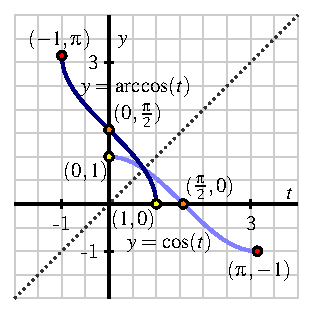
\includegraphics[width=0.8\linewidth]{inverse-trig-arccos-graph.png}
\end{image}
\end{callout}

Just as the natural logarithm function allowed us to rewrite exponential equations in an equivalent way (for instance, $y = e^t$ and $t = \ln(y)$ give the same information), the arccosine function allows us to do likewise for certain angles and cosine outputs.  For instance, saying $\cos\big(\frac{\pi}{2}\big) = 0$ is the same as writing $\frac{\pi}{2} = \arccos(0)$, which reads ``$\frac{\pi}{2}$ is the angle whose cosine is $0$''.  Indeed, these relationships are reflected in the plot above, where we see that any point $(a,b)$ that lies on the graph of $y = \cos(t)$ corresponds to the point $(b,a)$ that lies on the graph of $y = \arccos(t)$.%

\section{Exploring Arccosine}

\begin{example}%
Use the special points on the unit circle to determine the exact values of each of the following numerical expressions.  Do so without using a computational device.%
\begin{enumerate}
%
\item $\cos\Big(\arccos\Big(-\frac{1}{2}\Big)\Big)$

\begin{explanation}
We start by finding $\arccos\Big(-\frac{1}{2}\Big)$. Remember that for $x$ in $[-1,1]$, $\arccos(x)$ is the angle $\theta$ in $[0,\pi]$ such that $\cos(\theta) = x$. Hence we are looking for the value of $\theta$ corresponding to the point on the upper hemisphere of the unit circle with $x$-value $-\frac{1}{2}$.

\begin{image}
\begin{tikzpicture}
	\begin{axis}[
            xmin=-1.1,xmax=1.1,ymin=-1.1,ymax=1.1,
            axis lines=center,
            width=4in,
            xtick={-1,1},
            ytick={-1,1},
            clip=false,
            unit vector ratio*=1 1 1,
            xlabel=$x$, ylabel=$y$,
            every axis y label/.style={at=(current axis.above origin),anchor=south},
            every axis x label/.style={at=(current axis.right of origin),anchor=west},
          ]        
          \addplot [dashed, smooth, domain=(0:360)] ({cos(x)},{sin(x)}); %% unit circle

          \addplot+[thick,penColor2,->] plot coordinates {(0,0) (-.5,.866)}; %% 120 degrees

          \addplot+[thick,penColor,->] plot coordinates {(0,0) (1,0)}; %
          
          \addplot [textColor,smooth, domain=(0:120)] ({.15*cos(x)},{.15*sin(x)});
          \node at (axis cs:.01,.07) [anchor=west] {$\theta$};
	 \addplot+[penColor2, soliddot] coordinates{(-.5,.866)};
          \node[penColor3] at (axis cs:-.5,.866) [above left] {$\Big(\!\!-\frac{1}{2},\sin(\theta)\Big)$};         
         \end{axis}
\end{tikzpicture}
\end{image}

Hence, $\theta$ is $\frac{2\pi}{3}$, and we now see that 
\begin{equation*}
\cos\Big(\arccos\Big(\!-\frac{1}{2}\Big)\Big) = \cos\Big(\frac{2\pi}{3}\Big) = - \frac{1}{2}.
\end{equation*}

Now, if you're thinking, ``Hey, we didn't need that extra step!" Then you would be correct. But \textbf{\textit{why}} didn't we need that final step?

Let's recall how we defined arccosine. Since cosine is a periodic function, it fails the horizontal line test. However, if we {\it restrict} cosine to a portion of its domain on which it is only decreasing, $[0,\pi]$, then we may define a function $g$ on this domain such that $g(x) = \cos(x)$ for $x$ in $[0,\pi]$. Arccosine is defined as the inverse of this function $g$. Therefore, $g$ is the inverse of arccosine. 
Thus, in practice, cosine is the inverse of arccosine. 

A word of caution: arccosine is only the inverse of restricted cosine, as we will demonstrate with the next example.

\end{explanation}
%
\item $\arccos\Big(\cos\Big(\frac{7\pi}{6}\Big)\Big)$

\begin{explanation}
It may be tempting to take a look at this expression and conclude that the solution is $\frac{7\pi}{6}$ since arccosine is the inverse of cosine. 

{\bf But wait! }

Remember, we had to restrict the domain of cosine in order to define an inverse function, which we called arccosine. Arccosine is the inverse of the {\it restricted} cosine function, whose domain is $[0,\pi]$. $\frac{7\pi}{6}$ is larger than $\pi$, so it is not within the domain of this restricted cosine. 

Thus, we begin by simplifying $\cos\Big(\frac{7\pi}{6}\Big) = -\frac{\sqrt{3}}{2}$. 

Now, when we consider $\arccos\Big(-\frac{\sqrt{3}}{2}\Big)$, we will once again recall the unit circle. We are looking at the upper hemisphere, but this time we want to find the angle $\theta$ in $[0,\pi]$ that corresponds to the point with $x$-value $-\frac{\sqrt{3}}{2}$.
%
\begin{image}
\begin{tikzpicture}
	\begin{axis}[
            xmin=-1.1,xmax=1.1,ymin=-1.1,ymax=1.1,
            axis lines=center,
            width=4in,
            xtick={-1,1},
            ytick={-1,1},
            clip=false,
            unit vector ratio*=1 1 1,
            xlabel=$x$, ylabel=$y$,
            every axis y label/.style={at=(current axis.above origin),anchor=south},
            every axis x label/.style={at=(current axis.right of origin),anchor=west},
          ]        
          \addplot [dashed, smooth, domain=(0:360)] ({cos(x)},{sin(x)}); %% unit circle

          \addplot+[thick,penColor2,->] plot coordinates {(0,0) (-.866,.5)}; %% 150 degrees

          \addplot+[thick,penColor,->] plot coordinates {(0,0) (1,0)}; %
          
          \addplot [textColor,smooth, domain=(0:150)] ({.15*cos(x)},{.15*sin(x)});
          \node at (axis cs:.01,.07) [anchor=west] {$\theta$};
	 \addplot+[penColor2, soliddot] coordinates{(-.866, .5)};
          \node[penColor3] at (axis cs:-.824,.51) [above] {$\Big(\!\!-\!\frac{\sqrt{3}}{2},\sin(\theta)\!\Big)$};         
         \end{axis}
\end{tikzpicture}
\end{image}
%
Hence, $\theta$ is $\frac{5\pi}{6}$, and we now see that 
\begin{equation*}
\arccos\Big(\cos\Big(\frac{7\pi}{6}\Big)\Big) = \arccos\Big(\!-\frac{\sqrt{3}}{2}\Big) = \frac{5\pi}{6}.
\end{equation*}

Now, let's look again at the graph of cosine. Here we highlight $g: [0,\pi] \rightarrow [0,\pi]$ defined by $y=g(x)=\cos(x)$, the restricted cosine function. We may use the symmetry of the graph of cosine to help find the appropriate values for arccosine.
\begin{image}
\includegraphics[width=0.8\linewidth]{inverse-trig-PA-cosine.png}
\end{image}


%Something about arccos reflecting over the x-axis...
%add in graph of cosine and highlight the relevant part to avoid going back to other part...so symmetry of cosine graph--no more circles
%In Homework: Could do something like "should we expect a 'number' or an 'angle' when taking arccosine (or cosine) of something?"?  That often has been helpful.   And that arccosine will always put us in QI or QII only. --careful with angle eg, arcsine of sine of 3
%A good "trick" question would be cosine of 1/SQRT(2) or arccosinE of pi/4.


\end{explanation}

\item We can also solve trig equations as in the section Some Applications of Trig Functions. Solve the equation $4\arccos(x)-3\pi=0$.

\begin{explanation}
We start by isolating the arccosine term so that our equation is now
$$\arccos(x) = \frac{3\pi}{4}.$$

We observe that $\frac{3\pi}{4}$ is in the range of arccosine, so we may use the fact that cosine is the inverse of arccosine. Thus, $\arccos(x) = \frac{3\pi}{4}$ is equivalent to 
$$\cos(\arccos(x)) = \cos\bigg(\frac{3\pi}{4}\bigg).$$
%
This is further equivalent to $x = -\frac{\sqrt{2}}{2}$.
\end{explanation}
%
\end{enumerate}
\end{example}



%\begin{example}
%A standard example with solution in the text.
%	\begin{explanation}
%	Every example should have an explanation.
%	\end{explanation}
%\end{example}
%


\begin{summary}
  %Often ends a section
  \begin{itemize}
\item Any function that fails the Horizontal Line Test cannot have an inverse function.  However, for a periodic function that fails the horizontal line test, if we restrict the domain of the function to an interval that is the length of a single period of the function, we then determine a related function that does, in fact, have an inverse function.  This makes it possible for us to develop the inverse function of the restricted cosine function.
\item We choose to define the restricted cosine function on the domain $[0,\pi]$. On this interval, the restricted function is strictly decreasing, and thus has an inverse function.  The restricted cosine function has range $[-1,1]$. 
  \end{itemize}
\end{summary}


\end{document}
